\chapter{Reference Orientations} \label{chap:orientations}

The order of the vertices of a $n$-cell implicitly determines the boundary $k$-cells,
thus it is crucial to provide the vertices in the correct order.
While one- and two-dimensional objects provide little space for variations of reference orientations,
the situation changes in higher dimensions. The reference orientations
of the boundary $k$-cells provides ample of variations, while only a few choices
satisfy requirements such as consistent cell normals.

The reference orientations in {\ViennaGrid} are chosen such that the tuples
of vertex IDs for all boundary cells are in ascending order. This is accomplished
in a generic way for a unit-$n$-cell from the simplex and hypercube families in the $n$-dimensional space as follows:
\begin{enumerate}
 \item Start with a $1$-cell at the points $(1, 0, \ldots)$ and $(0, 1, 0, \ldots)$, enumerate the points and set $k=2$.
 \item Prolongate the $k-1$-cell to a $k$-cell in the $k$-dimensional subspace induced by the first $k$ unit vectors.
 \item Enumerate the new vertices.
 \item If $k=n$, stop. Otherwise, go back to $2$.
\end{enumerate}

The families of simplices and hypercubes differ in the way the the prolongation is carried out.
Details are given in the following subsections.

Boundary $k$-cells are ordered with respect to the less-than operator acting on the tuple of vertices in ascending order.
The first entry has precedence over the second entry, etc.

\section{Simplices}
\begin{figure}[tb]
\centering
 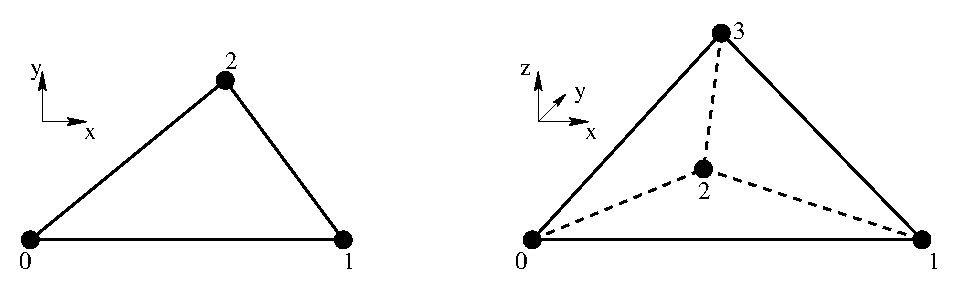
\includegraphics[width=0.7\textwidth]{figures/orientation-simplex.eps}
 \caption{Reference orientations of a triangle (left) and a tetrahedron (right).}
 \label{fig:orientation-simplex}
\end{figure}

The prolongation from a $k-1$-simplex to a $k$-simplex is straightforward, since only one vertex is added.
Resulting reference orientations for a triangle and a tetrahedron are given in Fig.~\ref{fig:orientation-simplex}.

Boundary $k$-cell orientations are chosen such that the tuple of vertices is sorted in increasing order.
Note that this does not lead to a consistent orientation of $n$-cell normals. In particular,
the boundary $k$-cells of a triangle and a tetrahedron are thus ordered as follows:
\begin{center}
 \begin{tabular}{|l|c|c|}
  \hline
              & Triangle                  & Tetrahedron   \\
  \hline
   $1$-cells  & $[0,1]$, $[0,2]$, $[1,2]$ & $[0, 1]$, $[0, 2]$, $[0,3]$, \\
              &                           & $[1, 2]$, $[1, 3]$, $[2,3]$ \\
  \hline
   $2$-cells  & $[0,1,2]$                 & $[0,1,2]$, $[0,1,3]$, \\
              &                           & $[0,2,3]$, $[1,2,3]$ \\
  \hline
 \end{tabular}

\end{center}


\section{Hypercube}
\begin{figure}[tb]
\centering
 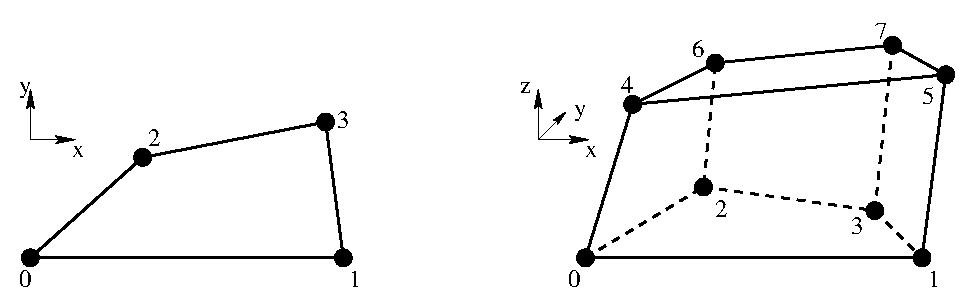
\includegraphics[width=0.7\textwidth]{figures/orientation-hypercube.eps}
 \caption{Reference orientations of a quadrilateral (left) and a hexahedron (right).}
 \label{fig:orientation-hypercube}
\end{figure}

For the prolongation from a unit-$k-1$-hypercube to a unit-$k$-hypercube, the standard tensor
construction is used. This results in a second $k-1$-hypercube shifted along the $k$-th unit vector,
with the new vertices enumerated in the same orientation as the initial $k-1$-hypercube.
This procedure can also be seen in Fig.~\ref{fig:orientation-hypercube}, where 
the two $1$-cells used for the prolongation to the hexahedron are $[0,1,2,3]$ and $[4,5,6,7]$.

For reference, the edges and faces of a quadrilateral and a hexahedron are ordered as follows:
\begin{center}
 \begin{tabular}{|l|c|c|}
  \hline
              & Quadrilateral                      & Hexahedron   \\
  \hline
   $1$-cells  & $[0,1]$, $[0,2]$, $[1,3]$, $[2,3]$ & $[0,1]$, $[0,2]$, $[0,4]$, $[1,3]$, $[1,5]$, $[2,3]$, \\
              &                                    & $[2,6]$, $[3,7]$, $[4,5]$, $[4,6]$, $[5,7]$, $[6,7]$ \\
  \hline
   $2$-cells  & $[0,1,2,3]$                        & $[0,1,2,3]$, $[0,1,4,5]$, $[0,2,4,6]$, \\
              &                                    & $[1,3,5,7]$, $[2,3,6,7]$, $[4,5,6,7]$ \\
  \hline
 \end{tabular}

\end{center}

\NOTE{Mind that the the reference orientations of a {\ViennaGrid} quadrilateral and a {\ViennaGrid} hexahedron coincide with those of the VTK types \lstinline|VTK_PIXEL| and \lstinline|VTK_VOXEL|, but differ from the orientations of the VTK types \lstinline|VTK_QUAD| and \lstinline|VTK_HEXAHEDRON|.}

